% !TEX root = ../main.tex
%
\chapter{Technical Implementation}
\label{sec:system}

\section{System Architecture}
\label{sec:system:architecture}

% Technology Stack Rational
% Architecture Diagram & data flow

The architecture followed a standard client server pattern, with the server functioning as a wrapper for the nerfstudio CLI, and the client as a web application.
The server is responsible for handling incoming requests from the client, and translating them into commands that the nerfstudio CLI could understand.
Requests from the client were sent to the server using HTTP requests, and in case of an asynchronous operation, the server would update the client on using websockets.

\begin{figure}[htb]
	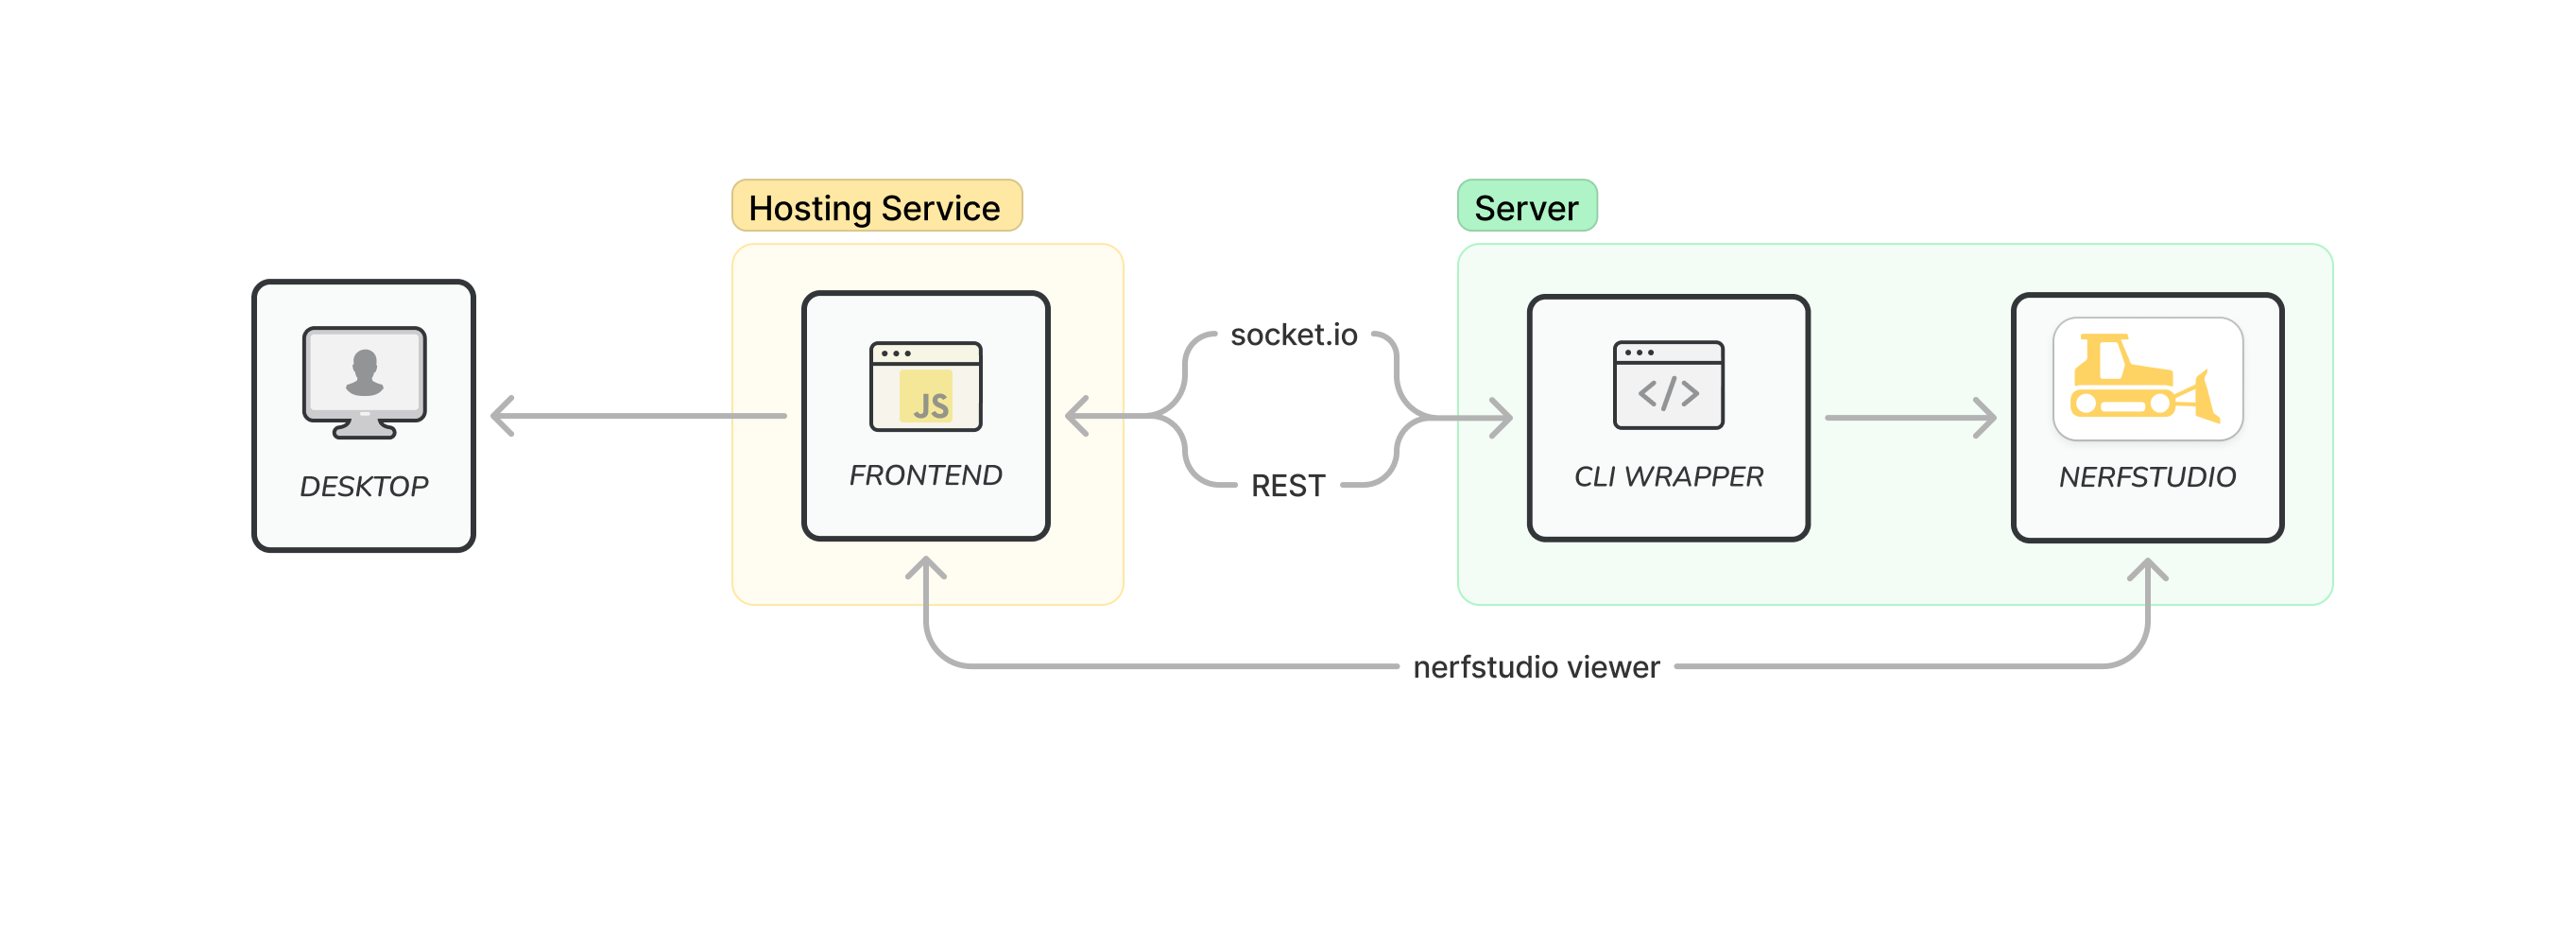
\includegraphics[width=\textwidth]{figures/architecture-1.png}
	\caption{System Architecture}
	\label{fig:system:example2}
\end{figure}

For the prototype, all the components were composed into a single docker container and deployed as a single unit.
This leveraged the pre-configured container provided by nerfstudio, and allowed for a quick and easy deployment of the prototype.

\section{Frontend Development} 
\label{sec:system:frontend}

% Setup, configuration, and component architecture
% UI/UX design principles

The frontend was built with React \cite{noauthor_react_nodate}, as it is a popular and well supported framework for building web applications.
Vite \cite{noauthor_vite_nodate} was used as a build tool, as it provides a fast and efficient development experience.
To accelerate the styling process, Tailwind CSS \cite{noauthor_tailwind_2020} was used, it is a utility-first CSS framework that provides a set of pre-defined classes that can be used to style components.
In additional the daisyUI \cite{noauthor_daisyui_nodate} component library provided a set of pre-styled components that could be used to quickly build the UI.

\subsubsection{Extensibility}

Extensibility was a key considerations during the development of the frontend, as the underlying nerfstudio CLI is in itself extendable.
All parameters for processing and training a NeRF model are configurable using JSON or strongly typed TypeScript objects.

\begin{lstlisting}[style=ES6, caption=Parameter Option configuration]
const stepsPerSave: NumberInput = {
	name: "stepsPerSave",
	label: "Steps Per Save",
	tooltip: "Number of steps between each save of the model.",
	inputType: "number",
	defaultValue: 1000,
};
\end{lstlisting}

Currently the supported input types are: number, select and boolean, but it is easy to add new types by extending the configuration object. 
It is also possible to define dependent parameters, that are only shown when a certain condition is met.
Images to illustrate the effect of a parameter can be added as well, to provide additional context to the user.

Filters and presets are also configurable using arrays of the names of the parameters that should be included in the filter or preset.
The full configuration can be found in the \texttt{frontend/src/config} folder in the codebase.

\subsubsection{Nerfstudio Viewer Integration}

The nerfstudio viewer is built using Viser \cite{noauthor_nerfstudio-projectviser_2024}, a library for building 3D visualizations using python.
This posed some limitations in integrating it into the frontend, as it is not easily possible to directly embed a python application into a web application.
To work around this, the viewer was hosted by nerfstudio and embedded into the frontend using an iframe.

Some modifications could be made to the viewer to make it more suitable for embedding.
This included some simple styling changes to make the viewer fit better into the frontend.
More complex changes were also made to improve the user experience.
The viewer contained several interactions where it was necessary for the user to copy console commands, to be used in the CLI.
These interactions were replaced with buttons that send a request to the server to execute the command instead.

This main shortcoming of this approach is that the frontend is unaware of the state of the viewer, and cannot update the UI based on action triggered in the viewer. 
It has to rely on polling the server to get the current state of rendering processes to give feedback to the user.

These modifications were done at build-time of the container by applying a patch to the nerfstudio source code of the base image.


\section{Backend Development}
\label{sec:system:backend}

% Advantages of tRPC, configuration, and API design

The backend was built using tRPC \cite{noauthor_trpc_nodate}, a framework for building type-safe APIs in TypeScript.
This type-safety was useful in building the API, as nerfstudio endpoints require a specific set of parameters of various types, that could be easily defined using TypeScript and reused in the frontend.

A major concern for the backend was the handling of asynchronous operations.
Processes can often take several minutes to complete, and the user should be able to see the progress of these operations.
TRPC implements a feature called subscriptions, which allows the client to subscribe to a certain event, and receive updates when that event occurs.
This is used for any long running operations, such as pre-processing or training a NeRF model.

Some additional endpoints were implement using Express. 
This includes the file upload endpoint, which is used to upload images and videos to the server. 
As well as the render endpoint, called through the viewer, as there does not exist a tRPC client for Python. 

\begin{lstlisting}[style=ES6, caption=Example tRPC endpoint for Pre-Processing]
export const nerfstudioRouter = router({
	process: publicProcedure
		.input(
			z.object({
				project: z.string(),
				dataType: z.enum(["images", "video"]),
				...
			}),
		)
		.subscription(({ input }) => {
			return observable<{message: string}>((emit) => {
				const args = ...
				const process = spawn("ns-process-data", args, {
          cwd: path.join(WORKSPACE, input.project),
        })
				process.stdout.on("data", (data: any) => {
					emit.next({message: data.toString()});
				});
			});
		})
});
\end{lstlisting}

All project related data is stored in a workspace directory, which is mounted as a volume in the docker container. 
This allows for the data to persist between container restarts, and for the user to access the data outside of the container.

\section{Challenges and Solutions}
\label{sec:system:challenges}

\subsection{Limitations of tRPC}

Although tRPC is a powerful tool for building APIs, with tight a tight integration into the frontend, it is not without its limitations.

It lacks to the support of \texttt{multipart/form-data} file uploads, which are necessary for uploading images and videos.
This was solved by implementing a separate endpoint using Express, which is used to upload files to the server.

The way tRPC handles subscriptions is also not ideal for long running processes.
If the client disconnects, the subscription is lost, and the client will lose the context for incoming events.
A better solution could use a standard websocket connection, with the the events containing the state necessary for the client to properly update the UI.

As mentioned above, tRPC does not have a client for Python, which is necessary for the viewer. 
This required the implementation of another separate endpoint using Express, which is called by the viewer to render the NeRF model.

All these limitations could be solved by using a more general purpose framework, such as Express.

\subsection{Working with the nerfstudio CLI}

Building the prototype against the nerfstudio CLI offered a useful layer of abstraction.
This enabled rapid development, without having to worry about the underlying implementation details of a huge codebase.
However, this abstraction comes at the cost of flexibility and overall complexity of the system.

The CLI is built using tyro \cite{yi_brentyityro_2024}, a tool for building command line interfaces in Python using configuration objects.
Efforts were made to translate the configuration objects into TypeScript objects, that could be used throughout the project.
This would allow for a more seamless integration of the CLI.
Sadly this was not possible, as the configuration objects are not easily serializable, and would require a lot of additional work to implement.

Thus the implemented solution has to rely on manually constructing the commands based on documentation, which is error prone and not very maintainable.


\section{Lessons Learned}
\label{sec:system:lessons}

\section{Future Directions}
\label{sec:system:future}

\subsection{Improved CLI Integration}

As outlined above the approach of wrapping the nerfstudio CLI with a custom API has some limitations.
A more integrated and robust solution would be built within the nerfstudio codebase itself.

A possible solution might be able to re-use the existing configuration object, used for CLI, to build a REST API.
This would allow for a more seamless integration of the CLI into the frontend, and would allow for more flexibility in the future.
It would also reduce the overall complexity of the system, as it would not require a separate server to handle requests.

\subsection{Improved Viewer Integration}

The current approach of embedding the viewer in an iframe is not ideal.
The nerfstudio viewer in version 0.3.4 and earlier, was built using React with a direct integration of Viser.
With the first major release of nerfstudio, the viewer was rewritten in Python, and the React integration was removed.

Re-building this projects frontend with a framework such as Viser, would be very limiting in terms of features and flexibility.
A better solution would be to integrate Viser into the frontend, akin to the original nerfstudio viewer.
This integration would allow for a more seamless interaction between the frontend and the viewer, and improve the overall user experience.
UI elements could be re-used to ensure a consistent look and feel, and the frontend could react to events triggered in the viewer.

